\documentclass{article}

\usepackage[a4paper]{geometry}
\usepackage{amsmath, amssymb}
\usepackage{graphicx}
\usepackage{wrapfig}
\usepackage{color}
\usepackage[usenames,dvipsnames]{xcolor}
\usepackage{float}
\usepackage{setspace}

\title{\Huge Simulation of a Quantum Computer}

\author{Roshenac Mitchell \and Max Nolte \and Martin R\"{u}fenacht \and Mark Stringer \and Justs Zari\c{n}\u{s} }

%new commands
\newcommand{\ket}[1]{\left| #1 \right>}
\newcommand{\bra}[1]{\left< #1 \right|}
\newcommand{\braket}[2]{\left< #1 \vphantom{#2} \right|\left.\!\!\!\;#2 \vphantom{#1} \right>}

\setlength{\topmargin}{0in}

\begin{document}

\maketitle

\vfill

\begin{onehalfspace}

\begin{abstract}
A simulation of a quantum computer was implemented on a classical computer using the Java programming language. All basic components of a quantum computer were created and the Deutsch-Jozsa algorithm, Grover's quantum search algorithm and Shor's integer factorisation algorithm were implemented and successfully run. Shor's algorithm was used to factor 15 and 21 into their primes using a personal computer.
\end{abstract}

\vspace{50mm}

\begin{center}
Junior Honours Computational Physics Project

School of Physics and Astronomy, University of Edinburgh
\end{center}

\thispagestyle{empty}

\clearpage

\tableofcontents
\thispagestyle{empty}

\clearpage

\setcounter{page}{1}

\section{Introduction}
A classical computer that runs on electrical signals going around circuits has matured significantly since its inception and now forms the backbone of society. However, society has grown as well, along with its needs for more and more computing power. Transistors become smaller and armies of cores work in parallel to keep up with current demands. This trend can still continue for a while and it should work, but perhaps some lateral thinking is needed for the next step. That new idea could be a whole different approach: a quantum computer.

At the start of the 1980's Richard Feynman introduced his idea of a universal quantum computer. He realized that a quantum-mechanical system cannot really be simulated by a classical computer, only with an exponential slowdown. This would mean that a quantum computer can simulate a quantum mechanical system far more efficiently than a classical computer \cite{feynman1982}.

As the years went by, a number of algorithms suitable for a quantum computing machine were created. In 1992 Deutsch and Jozsa discovered one of the first algorithms that run exponentially faster than the classical version. Two years later in 1994 Shor's quantum algorithm for factoring numbers was born. Afterwards Grover found an unsorted database search algorithm. All these showed an exponential speed increase over their classical equivalents, so clearly there is some merit to this idea. 

The goal of this project was to explore the theoretical framework of quantum computing. This was achieved by programming a simulation of a quantum computer in Java. After all, you can only be sure that you understand something if you can teach it to a computer. The project code contains basic mathematical tools and a universal set of gates plus some more for convenience; these are used to construct a circuit for Grover's, Shor's and Deutsch-Jozsa algorithms as a proof of concept.

This report covers the theory, principles of quantum computing and the building blocks of the algorithms. This is followed by an explanation of the overall design and implementation details of the core components, operators and algorithms. We further discuss the main results of the project, including successes and points of potential improvement.


\section{Theory}
\subsection{Basics of Quantum Computation}
In a quantum computer information is stored in so-called \emph{qubits} (quantum bits), an analogy to classical bits. A qubit is a microscopic two-state quantum mechanical system, for example an electron with spin up or spin down or a photon with two perpendicular polarization states. These two states represent the computational basis \( \{\ket{0},\ket{1}\} \). So instead of either representing 0 or 1 like a classical bit, a qubit can be in both states simultaneously (a superposition of two states), for example \( \ket{\psi} = \alpha \ket{0} + \beta \ket{1} \). The wave functions are normalized: \( |\alpha|^2+|\beta|^2=1 \)

Multiple qubits form a \emph{Quantum Register}. Quantum registers can store several numbers at the same time, i.e. the system can be in all classical states at once. A quantum register consisting of \emph{n} qubits thus has \(2^n\) possible states. A quantum register of size four could be in state \( \ket{0110} \) but also in all other \( 2^4 = 16 \) states \( \{\ket{0000},\ket{0001}...\ket{1110},\ket{1111}\} \) at the same time.

The most general state for a \emph{n} qubit quantum register is thus

\begin{equation}
 \sum_{\mathbf{x}\in\{0,1\}^n} \alpha_x\ket{\mathbf{x}}
\end{equation}

Manipulations on qubits are done by unitary operations, these can be performed by \emph{quantum logic gates}. All quantum gates are reversible, in contrast to classical computers. Several quantum logic gates form a quantum network.

The gates can be represented by \(2^n\) by \(2^n\) matrices (where \emph{n} is the size of the quantum register) which act on the computational basis.

The computational basis of a two-qubit quantum register would be \( \ket{00}, \ket{01}, \ket{10}, \ket{11} \} \). So a gate acting on a register in state \( \ket{00} \) would be equivalent to multiplying the matrix by the vector

\begin{equation}
 \ket{00} =\{\ket{0} \otimes \ket{0} = \begin{pmatrix} 1 \\ 0 \end{pmatrix} \otimes \begin{pmatrix} 1 \\ 0 \end{pmatrix} = \begin{pmatrix} 1 \\ 0\\0\\0 \end{pmatrix}
\end{equation}

There are many equivalent ways to write multiple-qubit states \( \ket{\mathbf{x}} \) where \( \mathbf{x} \in \{0,1 \}^n \). For example

\begin{equation}
 \ket{\mathbf{x}} = \ket{3} = \ket{011} = \ket{0} \otimes \ket{1} \otimes \ket{1}
\end{equation}

One of the fundamental gates is the Hadamard gate. It is a unitary gate acting on one qubit and can be represented by the two-by-two matrix 

\begin{equation}
 H = \frac{1}{\sqrt{2}}
  \begin{pmatrix} 1 & 1 \\ 1 & -1 \\ \end{pmatrix}
\end{equation}

acting on the computational basis \(\{\ket{0},\ket{1}\}\) of the qubit.

\begin{figure}[H]
	\centering
	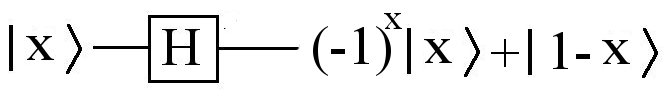
\includegraphics[width=50mm]{./images/hadamard}
	\caption{Graphical representation of the Hadamard gate}
\end{figure}

Another fundamental gate is the phase shift gate:

\begin{equation}
 \phi = \begin{pmatrix}	1 & 0 \\  0 & e^{ \imath \phi } \\ \end{pmatrix}
\end{equation}

A combination of two Hadamard and two phase shift gates can construct any unitary operation on a single qubit.

The phase shift gate is used in the Quantum Fourier Transform (QFT), a discrete Fourier transform applied to a quantum register. One of its uses is in Shor's algorithm, to put a quantum register in the superposition of all its states.

Thus for a quantum computer consisting of a single qubit the Hadamard and phase gate would be a universal set of operators, but a single qubit computer would not be of much use as the power of quantum computing lies in the entanglement of the qubits. This entanglement is done by multi-qubit gates consisting of control and target qubits. The simplest two-qubit gate is the “controlled NOT” gate (or C-NOT). The C-NOT gate is the reversible version of the classical (irreversible) XOR gate. It is made reversible by keeping the value of the control qubit. It is represented by the matrix

\begin{equation}
 C = \begin{pmatrix}
	1 & 0 & 0 & 0 \\
 	0 & 1 & 0 & 0 \\
	0 & 0 & 0 & 1 \\
	0 & 0 & 1 & 0
 	\end{pmatrix}
\end{equation}

\noindent acting on the computational basis \(\{\ket{00},\ket{01},\ket{10},\ket{11}\}\).

Another important two qubit gate is the controlled-V gate. Any unitary transformation acting on any number of qubits can be constructed by a network of only Hadamard and controlled-V gates. The controlled-V gate is represented by the matrix

\begin{equation}
 V = \begin{pmatrix}
	1 & 0 & 0 & 0 \\
 	0 & 1 & 0 & 0 \\
	0 & 0 & 1 & 0 \\
	0 & 0 & 0 & i
	 \end{pmatrix}
\end{equation}

The C-NOT gate and the C-V gate are both of the form controlled U. A control qubit is left unchanged, and a target qubit will be changed if the control qubit is in state \(\ket{1}\).

\begin{figure}[H]
	\centering
	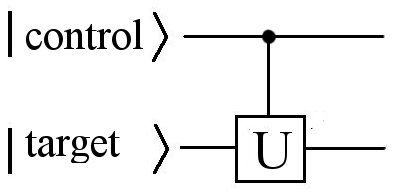
\includegraphics[width=35mm]{./images/cugate}
	\caption{Graphical representation of the controlled U gate}
\end{figure}

Another important gate for our simulation is the swap gate. It is a two-qubit gate that swaps two adjacent qubits and is represented by the matrix

\begin{equation}
 S = \begin{pmatrix}
	1 & 0 & 0 & 0 \\
 	0 & 0 & 1 & 0 \\
	0 & 1 & 0 & 0 \\
	0 & 0 & 0 & 1
 \end{pmatrix}
\end{equation}

The swap matrix can be used to swap qubits in a quantum register making control and target qubits adjacent. This helps when applying multiple-qubit gates like the C-NOT gate on non-adjacent qubits. The qubits can be swapped several times until they are adjacent. Then the C-NOT can be applied and afterwards they get swapped back to their original position. \cite{ekert2000, stolze2008}

\subsection{Algorithms}
\subsubsection{Deutsch-Jozsa Algorithm}
The Deutsch algorithm was originally set up for one qubit by Deutsch in 1985 and then generalized for any number of qubits by Deutsch and Jozsa in 1992 \cite{deutsch1985}. The algorithm has since been improved by R. Cleve et al., which is the version that is discussed here and implemented in the simulation \cite{cleve1998}.

The Deutsch-Jozsa algorithm determines whether a function \( f : \{0,1\}^n \to \{0,1\} \) inside a quantum computer oracle (\(U_f\)) is balanced or constant. If the function is constant, it will return either 0 or 1 for all possible inputs \( \{0,1\}^n\). If the function is balanced, it will return 0 for exactly \( 2^{n-1} \) combinations of \( \{0,1\}^n\) and 1 for the other \(  2^{n-1} \) combinations. The function is promised to be either constant or balanced and nothing else about it is known, it thus serves as a black-box. The internal structure of the function is irrelevant as long as it is either constant or balanced \cite{cleve1998,stolze2008}.

In the worst case, a classical computer would have to evaluate \(2^{n-1}+1\) combinations of \( \{0,1\}^n \) to get a deterministic answer (less for an answer with some uncertainty). The quantum algorithm however only needs a single evaluation to distinguish whether the function is constant or balanced and thus is exponentially faster than a classical computer.

The quantum mechanical function evaluation is implemented as a unitary transformation acting on the quantum register. There are \emph{n} input (control) qubits (the input to the function) and an addition (target) qubit to store the result of the evaluation: \\ \( U_f\ket{ \mathbf{x} , y} = \ket{ \mathbf{x} ,y \oplus f( \mathbf{x} ) }\) \footnote{The \(\oplus\) symbol denotes the exclusive or operation (XOR)} where \( x \in \{0,1\}^n , y  \in \{0,1\} \).

\begin{figure}[H]
	\centering
	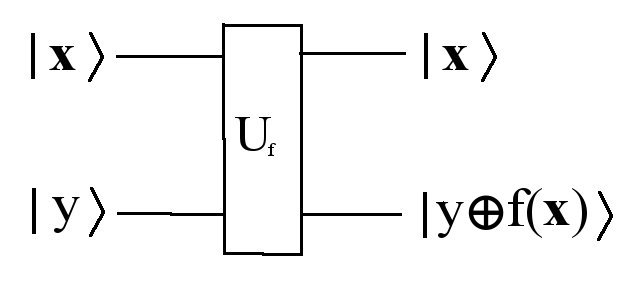
\includegraphics[width=45mm]{./images/deutsch1}
	\caption{Network representation of the oracle.}
\end{figure}

Thus the \emph{n} control qubits stay unchanged and the additional qubit is used to save the result. So for example if \( f(10110) = 1 \) \begin{displaymath} U_f|101101\rangle \to |101100\rangle  \end{displaymath}

\begin{figure}[H]
	\centering
	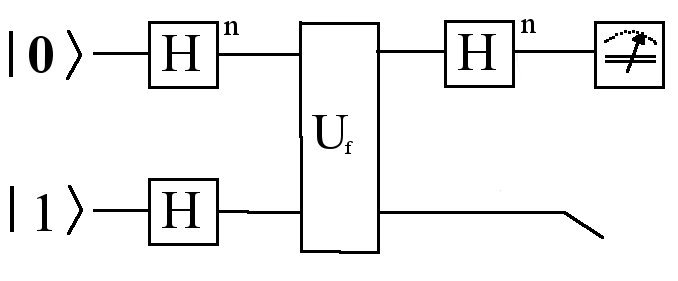
\includegraphics[width=50mm]{./images/deutsch2}
	\caption{Network representation of the Deutsch-Josza algorithm.}
\end{figure}

To run the algorithm, the register is initialized to the state \begin{math} \ket{\mathbf{x},y} = \ket{\mathbf{0},1}\end{math}, so all n control qubits are in state \(\ket{0}\) and the target qubit is in state \(\ket{1}\). A Hadamard gate is then applied to every single qubit causing the new state to be

\begin{equation}
 \frac{1}{\sqrt{2^{n+1}}} \sum_{\mathbf{x} \in \{0,1\}^n} \ket{\mathbf{x}} \otimes (\ket{0} - \ket{1}) 
\end{equation}


After applying the \(U_f\) gate this transforms to

\begin{equation}
 \frac{1}{\sqrt{2^{n+1}}} \sum_{\mathbf{x} \in \{0,1\}^n} (-1)^{f(\mathbf{x})} \ket{\mathbf{x}} \otimes (\ket{0} - \ket{1}) 
\end{equation}

Hadamard gates are then applied to the \emph{n} control qubits, but not to the target qubit, leading to

\begin{equation}
 \frac{1}{2^{n}} \sum_{\mathbf{x},\mathbf{z}\in\{0,1\}^n} (-1)^{f(\mathbf{x})\oplus (\mathbf{x} \cdot \mathbf{z})} |\mathbf{z} \rangle \otimes \frac{\ket{0} - \ket{1}}{\sqrt{2}}
\end{equation}

where \( \mathbf{x} \cdot \mathbf{z} \) is the scalar product modulo two. Now the amplitude of the state \begin{math} |\mathbf{z}\rangle = \ket{\mathbf{0}} \end{math} is 

\begin{equation}
 \sum_{\mathbf{x} \in\{0,1\}^n} \frac{(-1)^{f(\mathbf{x})}}{2^n}
\end{equation}

So if the function is balanced the \( (-1)^{ f( \mathbf{x} ) } \) terms will cancel and the amplitude of \(\ket{\mathbf{0}} = \ket{00...00}\) is zero. If the function is constant the terms will add up to \(\pm1\). Consequently a measurement of the \emph{n} control qubits will yield whether the function in the oracle is constant or balanced. It is constant if the measurement yields 0 and balanced for any other number\cite{cleve1998, stolze2008}.

\subsubsection{Grover's Algorithm}
Searching a unordered database in a classical computer is of \(O(N)\) complexity, where N is the number of entries, simply iterating through every item in the database and questioning the oracle; however in 1996 Lov Grover discovered a method of searching a database in \(O(\sqrt{N})\) complexity. The problem of searching a database is defined by finding the entry with the least amount of computational cost. Grover's algorithm is based on the fact that in a quantum computer it is possible to parallelise many queries to the oracle in a single step. This is very different compared to a classical algorithm which would require the oracle to be queried once for every item, hence the \(O(N)\) complexity. Grover went further than just discovering a search algorithm: he proved that it is impossible to accomplish this task in less time.

Grover's Algorithm consists of three main stages and results in a quantum register very likely to be the resulting answer we are looking for. These stages are:

\begin{enumerate}
 \item Initialisation
 \item Grover Iteration
	\begin{itemize}
		\item Oracle (\(U_w\)) 
		\item Diffusion Operator (\(U_s\)) 
	\end{itemize}
 \item Measurement
\end{enumerate}

The first stage, initialisation, sets the quantum register that will be acted upon into a complete superposition of all basis states. This is done by applying a Hadamard operator to each qubit within the quantum register. The resulting quantum register of this stage is \cite{lomo2000}:

\begin{equation}
 \ket{\psi} = \frac{1}{\sqrt{N}} \sum_{i=0}^{N-1} \ket{i}
\end{equation}

The second stage of Grover's Algorithm is the most complex of the three and involves mathematics that will not be covered \cite{lomo2000}, however final results will be given. During this stage an Oracle functioning in a way such that it can identify the answer (\(x_0\)) is required. The Oracle is a black box function which is represented by \cite{lomo2000}:

\begin{equation}
 f(x) = \left\{
	\begin{array}{lr}
		1 & if \: x = x_0 \\
		0 & otherwise
	\end{array}
	\right.
\end{equation}

The Oracle is a unitary transform of the quantum register it acts upon. The basis that represents the answer is phase shifted by \(\pi\), while the other bases are unchanged. Note that the phase shift does not have a classical analogue.

After the Oracle, another transform is applied: the Diffusion operator. This is defined by \cite{lomo2000}:

\begin{equation}
 U_s = -HI_{\ket{0}}H
\end{equation}

The Diffusion operator is unitary and is equivalent to an inversion about the mean values of the amplitudes of each state. In effect it increases the amplitude of \(\ket{x_0}\) and decreases the amplitude of the other bases.

By applying both the Oracle and the Diffusion operator a number of times to the resulting quantum register from the previous stage, the amplitude of the answer base increases. A representation of this process is a rotation of the quantum register in a two dimensional complex space from the initial superposition vector towards the \(\ket{x_0}\) basis. The number of steps required can be calculated by \cite{lomo2000}:

\begin{equation}
 k = \left \lfloor\frac{\pi}{4}\sqrt{N} \right \rfloor
\end{equation}

During the final stage of the algorithm, the resulting quantum register from the Grover iteration is measured, which causes it to collapsed into a specfic basis. This measurement results in a single base state with a non-zero amplitude and all other states with zero amplitudes, hence measuring again will always result in the same measurement. The probability that the answer state is obtained by the measurement is \cite{lomo2000}:

\begin{equation}
 Prob(\ket{x_0}) \geq 1 - \frac{1}{N}
\end{equation}

To test whether the correct result was retrieved the oracle can be queried to recognise the measurement, if it does not recognize it as the answer, the algorithm is restarted from the beginning.

Below is a graphical representation of the change of probabilities during the application of Grover's Algorithm.

If we assume the required answer (marked state) is 4 with 8 different possible states. 

\begin{figure}[H]
	\centering
	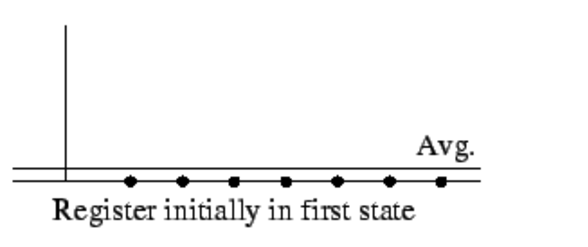
\includegraphics[width=70mm]{./images/grover_initial}
	\caption{The quantum register is initially prepared in the first state where base 0 has an amplitude of 1 and the rest have a zero amplitude. \cite{grovergraph} }
\end{figure}

\begin{figure}[H]
	\centering
	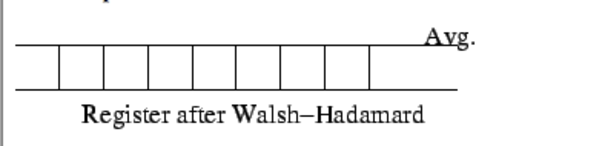
\includegraphics[width=70mm]{./images/grover_hadamard}
	\caption{A Hadamard gate is then applied which puts the QRegister into an equal superposition of all possible states. \cite{grovergraph}  }
\end{figure}

\begin{figure}[H]
	\centering
	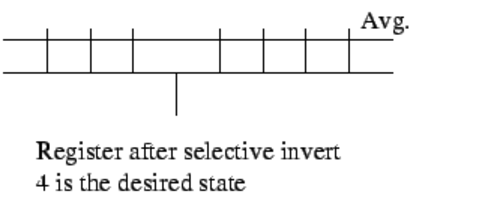
\includegraphics[width=70mm]{./images/grover_invert}
	\caption{When the Oracle is applied it goes through selective phase inversion. This switches the sign of the amplitude of the marked state. \cite{grovergraph} }
\end{figure}

\begin{figure}[H]
	\centering
	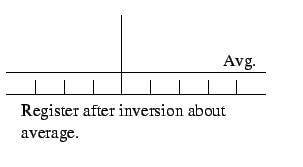
\includegraphics[width=70mm]{./images/afterinv}
	\caption{The Diffusion matrix then performs an inversion about average operation. This increases the amplitude of the state inverted in the previous step. \cite{grovergraph} }
\end{figure}

\subsubsection{Shor's Algorithm}
In the previous sections we have looked at two algorithms, Deutsch-Josza and Grover's: these have no real applications. In this section Shor's algorithm will be examined and its applications considered.

Shor's algorithm factors a number into its primes. It works for all odd composite numbers noting that an even number always has 2 as a prime factor, so can be continually divided by 2 until it is odd. Then Shor's algorithm can be applied to find some other factors. This means any number can be factored into its primes.

On a classical computer factoring prime numbers is currently very slow. With the best classical algorithms available one can currently factor a number into it’s primes in sub-exponential time\footnote{This means the algorithm still slows down faster than a polynomial rate but is significantly faster than an exponentially growing algorithm}.  Shor's algorithm uses the fact that a quantum register can be in a superposition of various states. So a gate acting on the quantum register will essentially calculate a superposition of states corresponding to the superposition of states put into the gate and the particular function of the gate. Furthermore it is easy for one to put a quantum register into a superposition of all it’s possible states by applying the quantum Fourier transform to a quantum register in the state \(\ket{0}\). 

Currently a lot of security, namely RSA encryption relies on the fact that it is hard to factor a number into its prime factors, using a classical computer. It is used everywhere in modern cryptography, as part of a key exchange and authentication protocols, which in turn is used everywhere in network security. One can imagine it would be disastrous if there was an easy way to compromise this security with many internet services relying on it, such as online banking and commerce. So far it has only been possible to factor up to 15 \cite{expdemo,demoshor}, so RSA is very unlikely to be compromised due to Shor's algorithm currently.

Factoring a number \emph{N}, into it’s primes can be accomplished by choosing a random number that is relatively prime to N and then finding P (the period of the function) such that P satisfies:

\begin{equation}
 m^P = 1 \bmod N
\end{equation}

Where m is a randomly generated positive integer.

After generating a value of m one should construct two quantum registers, the first with L qubits where L is determined from the expression 

\begin{equation}
 N^2=Q=2^L=2N^2
\end{equation}

This will store the values of the arguments of the function 

\begin{equation}
 x \rightarrow m^x \bmod N
\end{equation}


The second quantum register will have \(\log_2 N\) qubits. It will store the values of the function for the corresponding arguments in the first quantum register. Initially the quantum registers should be set such that the first one is in state \( \ket{0000\ldots 00} \) and the second one in the state \( \ket{0000\ldots 01} \), or in states \( \ket{\mathbf{0}} \) and \( \ket{\mathbf{1}} \) in decimal notation.

Now applying the Quantum Fourier transform to the first register it becomes a superposition of all the possible states the quantum register can be in: this is done in preparation for the next step. This leaves the system in the state 

\begin{equation}
 \frac{1}{\sqrt{2^L}}\sum_{x=0}^{2^L} \ket{x}\ket{1}
\end{equation}

\begin{equation}
 \ket{x}\ket{1} \rightarrow \ket{x}\ket{m^x \bmod N}
\end{equation}

Applying the above gate to the above state, you obtain two quantum registers: the first containing the arguments of the function and the second containing the values of the function.

Finally the Fourier transform is applied to register number one again to give the final state of the system Register number one is then measured giving a value \emph{y} which can be used to find the period of the function.

Using this value of y the period of the function can be found using continued fractions \cite{lomo2002}. This involves dividing the output by the size of the first quantum register (note, this is the basis size not the number of qubits, so \(2^n\)), then finding the convergent of the continued fraction and testing the denominator to see if it satisfies the expression for the  period \(m^p = 1 \bmod N \). If the convergent becomes 0, without obtaining the period then you have to start again.  Also note that this part can be done on a classical computer, after the measurement the quantum computer is no longer needed. 

Next we need to check if the period is even: if it is we can carry on, if not then unfortunately one has to rerun the algorithm from the start, with a new value of m.

\begin{equation}
 m^p = 1 \bmod N
\end{equation}

It is obvious that the expression above is satisfied. Therefore subtracting one from both sides gives.

\begin{equation}
 m^p-1 = 0 \bmod N 
\end{equation}

It is also required that the period has to be even, so the expression can be factored to give.

\begin{equation}
 (m^{\frac{p}{2}}+1)(m^{\frac{p}{2}}-1)=0 \bmod N
\end{equation}

If either factor is equal to 0 then the other can be any number, so we require that both are non-zero. If this requirement is not fulfilled then one has to rerun the algorithm from the start.

If both are non-trivial factors (i.e. neither is zero) then we have the two factors being some factors of some multiple of N. Therefore calculating the greatest common divisor of one of the  factors and N (which can be done easily using Euclid's algorithm) we can obtain one of the factors, then the other can be found simply by dividing N by the first factor.

\begin{equation}
 factor1 = \gcd(m^{\frac{p}{2}}\pm1,N) 
\end{equation}

\begin{equation}
factor2 = \frac{N}{factor1} 
\end{equation}


The reason Shor's algorithm works is due to the Quantum Fourier Transform applied the second time. The values of x that correctly give the period of the function add up (interfere) constructively. This is due to the fact that the coefficients (\(\omega^{i x}\)) in the quantum Fourier transform are roots of unity, and therefore are a cyclic group. If one imagines these roots on the complex plane, one can see that the values of \(\omega^{iP} \) are all the same so the amplitudes add constructively giving a large amplitude when the Fourier transform is applied.  The values of x that are not periods of the function add up (interfere) “destructively”, this is due to the fact that when the Fourier transform is applied \(\omega^{ix} \) will be different roots of unity, therefore summing over them will give zero. This means when the register is measured with a high probability the output will be a value such that it can be used to find the period.


\section{Implementation}
\subsection{Design}
The design of the implemented quantum computer simulation is based on a library design pattern. As such there is no strict usage of the source code, a host program simply imports the packages it requires. The source code was packaged into discrete packages to enable maximum extensibility. Four main packages are contained in the project: \emph{Core, Core.Math, Operators} and \emph{Algorithms}. The \emph{Core} package contains the fundamental classes required to represent a quantum computer, with the \emph{Core.Math} package containing the mathematical structures required. The \emph{Operators} and \emph{Algorithms} packages are extensions of the \emph{Core} package, which implement common operators and algorithms on quantum computers.

The \emph{Core} package contains a single implementation: \emph{QRegister}, representing a quantum register and three interfaces, \emph{Operator, Algorithm, AlgorithmOutput}. The \emph{Operator} interface is a representation of a linear operator and its interaction with \emph{QRegister} objects. The \emph{Algorithm} interface is defined such that an \emph{Algorithm} has a run method, either classical or quantum. In combination with \emph{Algorithm} we needed a variable output type to be the result of all algorithms, the \emph{AlgorithmOutput} interface represents this in such a way that the only requirement of the output of an algorithm is that it has a human readable string associated with it.

\begin{figure}[H]
	\centering
	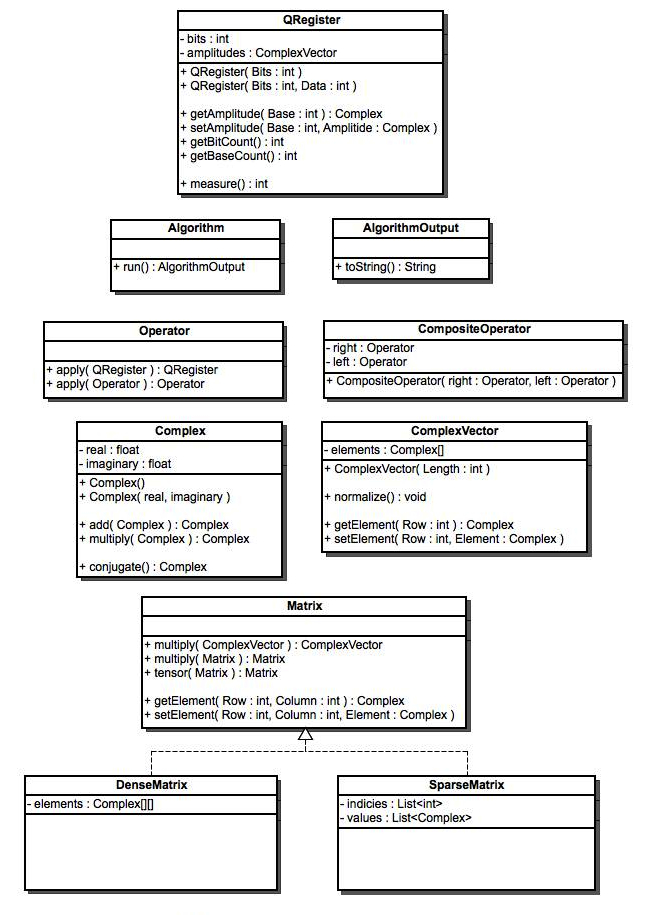
\includegraphics[width=140mm]{./images/design}
	\caption{UML description of the \emph{Core} package and \emph{Core.Math} package.}
\end{figure}

\subsection{Core}
The implementation of a quantum computer requires several classes such as \emph{Complex, ComplexVector} and \emph{Matrix} to do mathematical calculations. These were written with clarity in mind to provide a simple to use interface instead of a highly optimized one. While the \emph{ComplexVector} is simply an array of \emph{Complex} objects in combination with vector methods, the \emph{Matrix} class forms a class hierarchy of two implementations: \emph{DenseMatrix} and \emph{SparseMatrix}. Both represent a generic square matrix, however a \emph{DenseMatrix} has a complex element for each index while the \emph{SparseMatrix} is memory efficient. Two implementations were considered due to the fact that many of the unitary matrices are not very complex, in fact sparse. A factory method was created to allow switching between representations depending on a condition: If the number of non-zero elements in the matrix is above half the elements in the matrix then a \emph{DenseMatrix} representation would be used.


The \emph{QRegister} class is the only implemented class in the \emph{Core} package, since it represents the single data structure in a quantum computer. A quantum register is simply a complex vector that contains all the amplitudes in each eigenstate, therefore classical data would be represented as sparse vector. However this was not implemented since most algorithms initially put a zero quantum register into a superposition of all states which would be a dense representation. We implemented the \emph{QRegister} class as having an intrinsic ability to be measured, multiple methods are concerned with this topic.

Multiple situations arose during the project when input data could be corrupted in some form. As such we implemented an extension to Java's native exceptions to handle specific quantum computer exceptions and inform the user of errors without crashing the program.

\subsection{Operators}
In our simulator operators are defined by a single interface in the \emph{Core} package, they are declared to have two methods. The first method general to all operators is that they can be applied to a \emph{QRegister} object; the implementation of this method is dependent on the gate. The second method is an apply method to create a special operator type, \emph{CompositeOperator}, this method is general to the extent that it simply acts on the \emph{Operator} interface and needs no specific information about the implementation of \emph{Operator} it is acting on. By using the \emph{CompositeOperator} to create a tree of \emph{Operators} it is possible to have a single \emph{CompositeOperator} represent entire circuits.

We implemented many common operators that come up in quantum computing such as the \emph{Hadamard} operator, \emph{controlled-V} operator, \emph{phase shift} operator and more. Since the implementation of the operators is left to a subclass in the design most operators were designed to be an abstract class implementing the \emph{Operator} interface. All operators have their individual packages within the \emph{Operators} package and are implemented with either a matrix multiplication, a bit manipulation or a composite of other operators. Parameters required, such as target bit location or control bit location, are accepted through constructors of the base classes. As an alternative to a bit assignment operator an \emph{Operator} is completely responsible for required input and validity of it. This behaviour was chosen, because a bit assignment operator would allow for a generic operator to be applied to a \emph{QRegister} without information needed for functionality of that operator.

\begin{figure}
	\centering

	\begin{tabular}{ | c || c | c | c | }
		\hline
		Operator & Matrix & Bit Manipulation & Composite \\
		\hline
		\hline
		Hadamard & \checkmark & \checkmark & \\
		\hline
		Phase & \checkmark & \checkmark & \\
		\hline
		cV & \checkmark & \checkmark & \\
		\hline
		Swap &  & \checkmark & \\
		\hline
		CNot & \checkmark & \checkmark &  \checkmark \\
		\hline
		CCNot & & & \checkmark \\
		\hline
	\end{tabular}

	\caption{ Operator implementations }	
\end{figure}

The matrix implementation of an operator involves storing a matrix in a defined order of bases, representing the specific transform to the \emph{QRegister} object that is performed. This buffered matrix is then multiplied with the \emph{ComplexVector} representing the \emph{QRegister} and transforms it into a \emph{ComplexVector} with the operator applied. Since most operators are sparse a matrix is very wasteful in memory\footnote{Memory usage of \emph{DenseMatrix} is O(\(2^{2n}\))} and clock cycles, where n is the number of qubits, even when our \emph{SparseMatrix} implementation is used. The matrix multiplication is the analytic method of computing a quantum result. As an alternative to matrix multiplication, a bit manipulation method was devised for most operators. This involves stepping through all bases in a \emph{QRegister} object and using the specific basis index to implement the equivalent transform that is applied by the matrix multiplication. This method leads to a much less memory intensive operator structure and to a O(\(N\)) complexity of the operators, where N is the number of bases, compared to the O(\(N^3\)) matrix multiplication complexity; therefore large \emph{QRegisters} are easily handled compared to when matrices are used. The last method of implementation was to compose complex operators of simpler operators that act as a universal set of gates to a quantum computer. Specifically the \emph{controlled-V} gate was implemented to allow a mathematically elegant universal set with \emph{Hadamard} operators\cite{ekert2000}. The \emph{CNotCompositeOperator} and \emph{CCNotCompositeOperator} were both implemented in such a fashion to demonstrate this concept. Using the bit manipulation implementations of the universal set operators, a very efficient method arose to generate complex operators such as the \emph{CCNot} (Toffoli) operator. 

\subsection{Algorithms}
\subsubsection{Deutsch-Jozsa Algorithm}
The algorithm is implemented using three classes: \emph{DeutschJoszaAlgorithm}, which contains the main algorithm set up; \emph{DeutschJoszaOracle}, which is the quantum gate representing (\( U_f \)) and contains the function; and \emph{DeutschJoszaOutput}, which contains the result, i.e. whether the function is constant or balanced.

When creating the oracle, the user can decide whether to create a constant or a balanced function. There are several balanced functions implemented, but the code needs to be changed to access them, as one balanced function is enough to demonstrate the algorithm.

The whole structure of the simulation is very close to the real implementation. Hadamard gates are applied to all qubits and then the \emph{DeutschJoszaOracle} gate (the transform \begin{math} U_f \end{math}) is applied to the whole register consisting of the \emph{n} input qubits and the additional output qubit. Only one \emph{QRegister} containing n+1 qubits is used.

The oracle gate uses direct bit manipulation and no matrix representation. The function \( f : \{0,1\}^n \to \{ 0,1 \} \) is separated from the apply-method (which represents \( U_f \) ), so it can be easily changed.
\subsubsection{Grover's Algorithm}
The Grover Algorithm was implemented by using multiple classes to represent elements within the algorithm. One such class is the \emph{GroverOracle} this is the equivalent to the Oracle in the Grover Iteration stage. The \emph{GroverOracle} contains the answer that the QRegister will be converged to and also supplies information about the answer, i.e. the number of qubits required to represent it in binary and the base count(\(2^n\)). We chose this design of the Oracle to semantically seperate it from Grover's Algorithm implementation.

Grover's Algorithm is implemented using two different approaches, \emph{GroverDiffusionAlgorithm} with an analytic approach using a matrix as a diffusion operator\cite{solca2008} and \emph{GroverOptAlgorithm} with a combintation of basewise operators to act on the \emph{QRegister}. Both of these implementation only differentiate in the second stage of the algorithm. \emph{GroverOptAlgorithm} is a more efficent implementation due to less memory usage of the operators and is more sequential and therefore less complex to understand.

As a final addition to the Grover's algorithm implementation we added \emph{GroverDisplay} to show the convergence towards the given answer from the \emph{GroverOracle}. The two dimensional basis that is shown is generated by a Gram-Schmidt orthogonalisation of the answer base and initial zero base. The varying colours in the graph represents different steps in the algorithm with the most recent step colored red. As shown the algorithm begins at the superposition base and rotates towards the final answer base.

\begin{figure}[H]
	\centering
	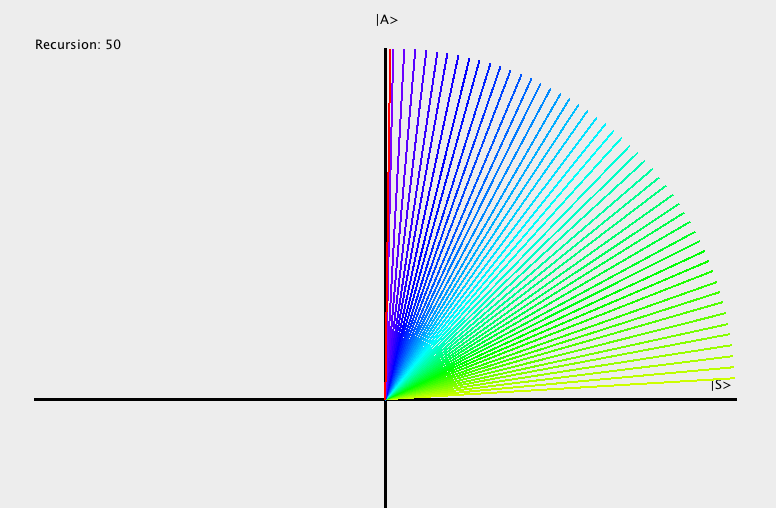
\includegraphics[width=80mm]{./images/GUI}
	\caption{GUI produced from \emph{GroverDisplay}. }
\end{figure}

\subsubsection{Shor's Algorithm}
We will now discuss how Shor's algorithm was implemented. We will initially talk about how the quantum part of the algorithm was implemented, and will move on to discuss how the classical part was implemented.

The quantum part of Shor's algorithm requires two gates: the Quantum Fourier Transform gate and the gate which applies the transform below

\begin{equation}
 \ket{x}\ket{1} \rightarrow \ket{x}\ket{m^x \bmod N}
\end{equation}

We chose to implement the Quantum Fourier Transform directly as a matrix, rather than using gates, as the matrix requires one initial calculation of omega and then omega raised to powers. It can be seen that the number of complex multiplications is

\begin{equation}
 ComplexMultiplications = \sum_{i,j=1} (i \cdot j) - 1
\end{equation}

\begin{equation}
 QFT_{2}=\begin{pmatrix}1 & 1 &1 &1 \\ 
 1 & \omega & \omega^{2} & \omega^{3} \\
 1 & \omega^{2} & \omega^{4} & \omega^{6} \\
 1 & \omega^{3} & \omega^{6} & \omega^{9} \end{pmatrix}
\end{equation}

Now, examining the gate construction, it is clear that  tensor products are required to calculate just the action of the first Hadamard gate, as a sparse matrix is not implemented in the gates  

\begin{equation}
 V =\sum_{l=0}^{p-2} k^{2(p-l)}
\end{equation}

Complex multiplications are required, where k is the order of the matrices (in this case 2) and p is the number of matrices being tensor produced together (which for Shor’s algorithm is Q). It is clear this is exponentially growing  (just from the first gate in the circuit), therefore creating the matrix from the methods above rather than gates is a much more efficient way to obtain the QFT. Hence this was used it in the simulation.

The gate that applies the transform \( \ket{x}\ket{1}\rightarrow\ket{x}\ket{m^x \bmod N} \)  was done simply by taking  the tensor product of the two quantum register state vectors, iterating through the possible values the first quantum register can hold, calculating the corresponding value of the function and setting the corresponding  components of the combined state vector to 1\footnote{As a quantum register is normalized when it is measured}.  It was decided to implement it this way as it was found to be very conceptually hard implementing this using just gates or a generating a matrix (if either is even possible for all n and m). We felt that a \emph{for} loop would be fine, and most likely would be faster than generating a matrix directly or using gates, then using matrix vector multiplication on the state vector.

The classical part was implemented directly in the Shor's algorithm method rather than in a separate class. It was chosen to implement it this way as it seems there are no other methods to reduce the quantum output to the period that is used: there was no need to separate it out, so it could easily be replaced.

In the algorithm above you can see there are many places the method could fail. For example: if the period is odd or  \( m^ {\frac{p}{2}}\pm1=0 \). To deal with this issue recursive relationships have been set up such that if the period fails to  satisfy one of its requirements, a message is printed out to the terminal saying it has failed. Then the output value for the method is set to the output of the method. This seems to have dealt with the problem in an elegant way however there is now risk of stack overflow occurring. This should not be an issue as Shor’s algorithm should find factors much quicker than the processor runs out of stack space.

During the testing process it was discovered that \emph{ints} were not large enough in the classical part, it was therefore decided to use \emph{BigIntegers} in the classical part.

Finally, If there was more time, a GUI could have been implemented to draw the probability distribution of the final state of the system to see which values are more likely. This would give a better understanding of how Shor's algorithm works and would allow us to check that the quantum part of the algorithm is working correctly easily.


\section{Discussion}
The finished code contains the basic mathematical tools of quantum computing and a large set of gates that are needed to build algorithms. These components have been used to implement Grover's, Shor's and Deutsch-Jozsa algorithms, thus proving the concept of a quantum computer. The algorithm frameworks and gates allow implementations of further algorithms and extensions to the simulation. The resulting packages are of significant value to test out ideas in theory before a complicated and expensive physical quantum system is built.

The things we did well were we adhering to good coding practices, i.e. a carefully planned out set of abstract classes. The use of version control system, \emph{GIT} in our case, allowed for efficient work. This and general organisational effort, like delegation of responsibilities, meant that there were almost no overlapping efforts and the code base quickly grew as we worked in parallel.

While an implementation of a quantum computer has been achieved, it is still rather limited in speed and memory capacity. As more qubits are added to the register, the memory and computation requirements grow exponentially. This is expected, though, as it is a simulation of a system in an incompatible environment, a quantum computer simulated on a classical computer, defeats the purpose. These difficulties arise because it is impossible to use the benefits that come with computations using particles and their quantum effects. Nature has infinite clock cycles.
Other difficulties were technical issues with the version control system which would frequently prohibit synchronisation of code possibly due to insufficient support from the IDE \emph{Netbeans}. There were also some naming convention inconsistencies that caused time loss as they had to be corrected in order to have coherent code.

The project was completed with a great deal of success but there is always room for improvement. For example, in the interest of completeness, more gates could have benefited from bit twiddling or otherwise more efficient implementations than matrix manipulation. The universal set, \emph{CNot} and \emph{Hadamard}, both have implementations so it is not a pressing issue.
The overall design is slightly circumvented by having a measure method hidden in the \emph{QRegister} class. The more consistent approach would be to have a separate measurement gate in the set of universal gates.
Another thing we could have implemented is a more intelligent matrix framework. For example a matrix that stores values in a set and then points to non-zero values in the actual matrix. This would allow matrices which do not have enough non-zero values to be sparse but enough equivalent elements to be represented well.
The naming convention inconsistencies could have been resolved by producing a sample class with every possible type of code in it. This would serve as a reference while writing code.



\section{Conclusion}
All components of a quantum computer have been successfully implemented in a Java simulation. With three working algorithms and a framework for extensions, the concept of quantum computing has been shown viable. We correctly implemented Deutsch-Jozsa, Grover's and Shor's algorithms. Using Shor's algorithm, 15 and 21 were factored effectively. By implementing operators in several different ways, performance and general memory usage have been improved throughout development.
\clearpage

\end{onehalfspace}

\bibliographystyle{unsrt}
\bibliography{references}

\end{document}